\mychapter{6}{Lesson 6} %181012

\section{Computationally secure encryption}

Having a better idea of what can and can't be accomplished in the cryptographic world, by means of theorems and proofs, we can focus now on the goal of defining a cryptographic system that meets our requirements. In this lesson, we focus specifically on the secrecy-oriented schemes, thus dealing with encryption and decryption of messages.

The requirements of a ``good'' encryption scheme are collectively called those of \emph{computationally secure encryption}: the characterizing requirement is to design a task, or routine, that is \emph{computationally hard} for an attacker to revert.
In detail: this task usually involves a secret key\footnotemark, and is accomplished in polynomial time, and any attacker who wishes to revert it has no efficient means of doing it without knowing such key. Other properties include:

\footnotetext{This is the case for symmetric-key schemes, though many other kinds exist: some involving ``public'' keys, some others not having any key at all}

\begin{enumerate}
    \item \label{prop:owk} \emph{one-way}ness with respect to the encryption key: given $c = \Enc(k, m)$, it should be hard to recover $k$
    \item \label{prop:owm} \emph{one-way}ness with respect to the original message: given $c = \Enc(k, m)$, it should be hard to recover $m$
    \item \label{prop:nol} In a stricter sense: no information whatsoever must ``leak'' from the message
\end{enumerate}

To start visualizing these concepts, let $\Pi = (\Enc, \Dec)$ be a secrecy scheme, and consider the game depicted in figure \ref{cryptogame:otindist}  where the adversary ``wins'' the game when the challenger outputs 1.

\begin{cryptogame}
    {otindist}
    {$\cryptog{ind}(\lambda, b)$}
    {ind}

    \send{}{$m_0, m_1 \in \M$}{}

    \receive{\shortstack[l]{
        $k \pickUAR \K$ \\
        $b \pickUAR \binary$ \\
        $c \pickUAR \Enc(k, m_b)$ }}
    {$c$}{}

    \cseqdelay

    \send{}{$b'$}{\textsc{Output 1 iff} $b = b'$}
    
\end{cryptogame}

\begin{definition}
    The scheme $\Pi$ is said to be \emph{computationally one-time secure} iff:
    \[
        \forall \adversary \in \ppt \implies \cryptog{ind}(\lambda, 0) \compindist \cryptog{ind}(\lambda, 1)\footnotemark
    \]  
    or, rephrased in probability terms:
    \[
        \forall \adversary \in \ppt \implies \lvert\Pr[\cryptog{ind}(\lambda, 0) = 1] - \Pr[\cryptog{ind}(\lambda, 1) = 1]\rvert \in \negl(\lambda) \qedhere
    \]
\end{definition}
\footnotetext{$\cryptog{ind}$ refers to the indistinguishability of the messages sent by \adversary{} during the game}

This last definition shows how such a scheme is compliant with the three properties exposed beforehand. In particular:

\begin{enumerate}
    \item \emph{It is hard to recover the key}. If not, then an adversary \adversary{} can efficiently recover the key and use it to decrypt the ciphertext, which in turn enables him to perfectly distinguish $m_{0}$ from $m_{1}$ on any instance;
    \item \emph{It is hard to recover the message}. This is analogous, and even more obvious than the preceding point. Nevertheless, this is a necessary condition for a secrecy scheme to be ``good'', and it mustn't be forgotten;
    \item \emph{No information about the message whatsoever may leak from the ciphertext}. This may seem subtler than the previous point, but it warrants caution. Observe how an adversary \adversary{}, if it has the ability to extract even a tiny bit of information of the original message from the ciphertext, then it is actually able to make an educated guess on which message was encrypted in the first place, putting him at an advantage. This leads the probabilities described in the definition to be sensibly more unbalanced than negligible, forfeiting the desired secrecy.
\end{enumerate}

By extension, we may ask ourselves what scheme may or may not be \emph{computationally two-time secure}. For instance, let $\Pi_{\oplus} = (\Enc, \Dec)$ be a secrecy scheme using a \prg{} $G : \binary^\lambda \to \binary^n$, structured as follows:

\begin{itemize}
    \item $\K = \binary^\lambda$, $\M = \C= \binary^n$
    \item $\Enc(k, m) = G(k) \oplus m$
    \item $\Dec(k, c) = c \oplus G(k) = m$
\end{itemize}

To be two-time secure means that, even if an adversary \adversary{} gets hold of a valid plaintext-ciphertext couple $(\overline{m}, \overline{c})$, he is unable to decrypt any future ciphertexts\footnotemark, apart from the obvious $\overline{c}$. However, observe that \adversary{} is now able to extract valuable information for decrypting future ciphertexts:

\footnotetext{This example models a technique called \emph{Chosen Plaintext Attack}, which will be discussed in depth later}

\[
    \overline{c} = \Enc(k, \overline{m}) = G(k) \oplus \overline{m} \implies \overline{c} \oplus \overline{m} = G(k)
\]
so now, for any second ciphertext \adversary{} receives, he can \emph{mimic} the decryption routine, and efficiently uncover the underlying plaintext. This proves that $\Pi_\oplus$ is not two time-secure; nevertheless, it is still one-time secure:

\begin{theorem}
    If $G$ is a \prg, then $\Pi_\oplus$ is computationally one-time secure
\end{theorem}

\begin{proof}
    This proof is another example that showcases the use of hybrid games. Recalling the one-time security definition, we need to show that:
    \[
        \forall \adversary \in \ppt \implies \cryptog{ind}[\Pi_\oplus](\lambda, 0) \compindist \cryptog{ind}[\Pi_\oplus](\lambda, 1)
    \]
    Consider the hybrid game in figure \ref{cryptogame:xorothybrid}, where the original encryption routine is changed to use a completely random value, instead of using $G(k)$\footnotemark. As an exercise, compare it with the original one-time secure definition in figure \ref{cryptogame:otindist}, to check that it perfectly matches.

    \footnotetext{The observant student may recognize that this modification yields exactly the ``one-time pad'' secrecy scheme discussed in lesson 1}

    \begin{cryptogame}
        {xorothybrid}
        {$\hybridg{}[\Pi_\oplus](\lambda, b)$}
        {r-ind}

        \send{$m_0 \neq m_1 \in \binary^l$}{$m_0, m_1$}{}

        \receive{\shortstack[l]{
            $r \pickUAR \binary^l$ \\   % R \sim \unifdist{\binary^l}
            $b \pickUAR \binary$ \\     % B \sim \unifdist{\binary}
            $c = r \oplus m_b$            % C = R \oplus m_B
        }}
        {$c$}{}

        \cseqdelay

        \send{}{$b'$}{\textsc{Output 1 iff} $b' = b$}
        
    \end{cryptogame}

    The proof begins by affirming that:
    \begin{claim}
        \[
            \forall \adversary \in \ppt \implies \hybridg{}[\Pi_\oplus](\lambda, 0) \equiv \hybridg{}[\Pi_\oplus](\lambda, 1)
        \]
    \end{claim}

    To prove it, notice that $r$ is chosen uniformly at random, and independently of $b$. Thus, no matter how the messages $m_0$ and $m_1$ are structured, $r$ will effectively make the chosen message completely unrecognizable. In formal terms, let $B$ and $R$ be the random variables for \challenger{}'s picks of $b$ and $r$ respectively; then:
    \begin{align*} % AP190906: Totally original, need a peer review here
        & \left| \Pr(B = 0 \knowing C = c) - \Pr(B = 1 \knowing C \evaluatesto c) \right| & \\
        =& \left| \Pr(B = 0 \knowing R \oplus m_B \evaluatesto c) - \Pr(B = 1 \knowing R \oplus m_B \evaluatesto c) \right| & \text{(C definition)} \\
        =& \mathrlap{\frac{\left| \Pr(R \oplus m_B = c \knowing B \evaluatesto 0) \Pr(B = 0) - \Pr(R \oplus m_B = c \knowing B \evaluatesto 1) \Pr(B = 1) \right|}{\Pr(R \oplus m_B = c)}} & \\
        & & \text{(Bayes' theorem)} \\
        =& \frac{\left| \Pr(R \oplus m_0 = c) \Pr(B = 0) - \Pr(R \oplus m_1 = c) \Pr(B = 1) \right|}{\Pr(R \oplus m_B = c)} & \text{(Cond. collapse)} \\
        =& \frac{\left| \oneover{2^l} \half - \oneover{2^l} \half \right|}{\Pr(R \oplus m_B = c)} = 0 & \\
    \end{align*}

    Having proven that \adversary's success is equivalent to straight guessing in $\hybridg{}[\Pi_\oplus]$, we now relate the hybrid game to the original one, affirming that:
    
    \begin{claim}
        \[
            \forall \adversary \in \ppt,\, \forall b \in \binary \implies \hybridg{}[\Pi_\oplus](\lambda, b) \compindist \cryptog{ind}[\Pi_\oplus](\lambda, b) \qedhere
        \]
    \end{claim}

    The proof proceeds by reduction as depicted in figure \ref{cryptoredux:xorotprg}, by assuming the existence of a distinguisher $\textsf{D}^{\textsc{ind}}$ for $c = G(k) \oplus m_{b}$ and $c = r \oplus m_{b}$, and using it to break $G$'s pseudo-random generation property.

    \begin{cryptoredux}
        {xorotprg}
        {Reducing to breaking a \prg}
        {prg}
        {G-ind}[2]

        \receive{\shortstack[l]{
            $k \pickUAR \binary^\lambda$ \\
            $x_0 \pickUAR G(k)$ \\
            $x_1 \pickUAR \binary^l$ \\
            $b \pickUAR \binary$
        }}{$x_b$}{}

        \return{}{$m_0, m_1$}{}

        \invoke{\shortstack[l]{
            $\beta \pickUAR \binary$ \\
            $c = x_b \oplus m_\beta$
        }}{$c$}{}

        \return{}{$\beta'$}{}

        \cseqdelay
        \send{$b' = \begin{cases}
            0 &\textsc{iff } \beta' = \beta \\
            1 &\textsc{else}
        \end{cases}$
        }{$b'$}{\textsc{Output 1 iff} $b' = b$}

    \end{cryptoredux}

    Again, notice how the games of indistinguishability and pseudo-random generation are reliably reproduced on their respective sides. This construct's value centers on how $\distinguisher^\textsc{ind}$ will perform in its own challenge:
    \begin{itemize}
        \item if $x_b$ is a random value, then $\distinguisher^\textsc{ind}$ will perform as depicted in the hybrid game, thus giving right or wrong answers at random;
        \item if b is the result of $G$, then $\distinguisher^\textsc{ind}$ has a better chance in finding the right answer by its own design;
    \end{itemize}
    From these observations, especially the second point, the adversary \adversary{} has a better chance of winning the \prg{} game by asserting that $x_b$ comes from $G$ whenever $\distinguisher^\textsc{ind}$ makes a correct guess; conversely, \adversary{} will preferably declare that $x_b$ is truly random whenever $\distinguisher^\textsc{ind}$ fails a guess, as the probability of the latter getting fooled by a random value is sensibly greater than by a pseudo-random one.

    Either way, by the existence of $\distinguisher{}^\textsc{ind}$, \adversary{} gains an edge in efficiently recognizing $G$, which cannot happen by $G$'s definition; the claim is proven. The theorem's proof can be completed by putting the pieces together, as is usual in the hybrid argument:
    \[
        \cryptog{ind}[\Pi_\oplus](\lambda, 0) \compindist
        \hybridg{}[\Pi_\oplus](\lambda, 0) \equiv
        \hybridg{}[\Pi_\oplus](\lambda, 1) \compindist
        \cryptog{ind}[\Pi_\oplus](\lambda, 1)
    \]

    which finally states that $\cryptog{ind}[\Pi_\oplus](\lambda, 0) \compindist \cryptog{ind}[\Pi_\oplus](\lambda, 1)$.
\end{proof}
 

\section{Pseudorandom functions}

\textsc{Prg}s are used in practice as a stepping stone for building \emph{pseudo-random functions}, \prf{} henceforth, which are the principal construct in several cryptographic schemes. Before formally introducing what a \prf{} is, we begin instead by defining what a \emph{truly random function} is:

\begin{definition}
    A random function $R : \binary^n \to \binary^l$ is a function that, depending on what is known about its previous applications:

    \begin{itemize}
        \item if $x$ is ``fresh'' (in formal terms, $R$ has never been applied to $x$ beforehand), then a value $y$ is chosen \uar{} from $R$'s codomain, and it is permanently associated as the image of $x$ in $R$\footnote{This property is also called \emph{lazy sampling}.};

        \item if $x$ is not fresh, then $R(x)$ is directly returned instead. \qedhere
    \end{itemize}
\end{definition}

It should be noted that, if such functions are to be implemented in computers, they would occupy too much space in memory. Suppose all the possible outputs of $R$ have been generated and stored as an array in memory; then its total size in bits will be $l \cdot 2^n$:

\[  
    \color{black!50}
    \overbracket[0.5pt][5pt]{\;\color{black}\framebox[4em][c]{0010...}\;}^{l \text{ bits}}_1\;
    \overbracket[0.5pt][5pt]{\;\color{black}\framebox[4em][c]{1110...}\;}^{l \text{ bits}}_2\;
    \overbracket[0.5pt][5pt]{\;\color{black}\framebox[4em][c]{0011...}\;}^{l \text{ bits}}_3\;\;
    \color{black!25}
    \framebox[2em][c]{\rule{0pt}{1.5ex}...}\;
    \framebox[2em][c]{\rule{0pt}{1.5ex}...}\;
    \framebox[2em][c]{\rule{0pt}{1.5ex}...}\;
    \framebox[2em][c]{\rule{0pt}{1.5ex}...}\;\;
    \color{black!50}
    \overbracket[0.5pt][5pt]{\;\color{black}\framebox[4em][c]{1110...}\;}^{l \text{ bits}}_{2^n}
\]

Such a function becomes cumbersome and difficult to maintain in practice; therefore, it is desirable to find a kind of function which looks as a random function possible, but does not require to be wholly memorized, while not forgetting to maintain poly-time complexity. Pseudo-randomness comes to the rescue here:

\begin{definition}
    Let $f$ be a function, then it is deemed pseudo-random (therefore, $f$ is a \prf{}) iff it is computationally indistinguishable from a true random function.
\end{definition}

In detail, \prf{}s are actually designed as function families $f_k$\footnotemark, where $k$ is a parameter that indexes the functions inside the family. To model the \prf{}s' indistinguishability from random functions, let $F \in \binary^\lambda \to (\binary^{n(\lambda)} \to \binary^{l(\lambda)} )$, usually denoted simply by $f_k$, be a \prf{}, and define $\mathfrak{R}(n, l)$ to be the domain that collects the random functions from $\binary^{n(\lambda)}$ to $\binary^{l(\lambda)}$.

\footnotetext{Does this remind you of something else? If not, look back in lesson 2 and 3.}

Consider the indistinguishability game drawn in figure \ref{cryptogame:prf}; although one may thing that \prg{}s and \prf{}s aren't much different, the game tells a different story, which is best put by an introductory paragraph about \prf{}s in their Wikipedia page:

\begin{quotation}
    ``Pseudorandom functions are not to be confused with pseudorandom generators (\prg{}s). The guarantee of a \prg{} is that a single output appears random if the input was chosen at random. On the other hand, the guarantee of a \prf{} is that all its outputs appear random, regardless of how the corresponding inputs were chosen, as long as the function was drawn at random from the \prf{} family.''\footnote{\linkicon \href
        {https://en.wikipedia.org/wiki/Pseudorandom_function_family}
        {\textsf{Pseudorandom function family --- Wikipedia}}}
\end{quotation}

\begin{cryptogame}
    {prf}
    {The \prf{} indistinguishability game}
    {prf}

    \cseqchallenger{\shortstack[l]{
        $k \pickUAR \binary^\lambda$ \\
        $R \pickUAR \mathfrak{R}(n, l)$ \\
        $b \pickUAR \binary$
    }}

    \cseqdelay
    \cseqbeginloop

    \send{}{$x$}{}

    \receive{\shortstack[l]{
        $y_0 = f_k(x)$ \\
        $y_1 = R(x)$
    }}{$y_b$}{}

    \cseqendloop
    \cseqdelay

    \send{}{$b'$}{\textsc{Output 1 iff} $b = b'$}

\end{cryptogame}

In this game, \adversary{} is allowed to make multiple queries to $\challenger^\prf$, as opposed to the \prg{} indistinguishability game where it can perform just one query before making its guess. To reiterate the \prf{} definition in terms of this game:

\begin{definition}
    A function family $F = f_k$ is a \prf{} iff: 
    \[
        \cryptog{prf}[f_k](\lambda, 0) \compindist \cryptog{prf}[f_k](\lambda, 1) \qedhere
    \]
\end{definition}

\begin{exercise}
    Prove the following statements:
    \begin{itemize}
        \item No \prg{} is secure against unbounded attackers;
        \item No \prf{} is secure against unbounded attackers.
    \end{itemize}
   
\end{exercise}


\subsection{\textsc{Ggm}-tree}

This section is dedicated to a concrete example of a \prf{} which is built from the ground up using a \prg. This construct has been designed from Oded Goldreich, Shafi Goldwasser and Silvio Micali, and its structure is akin to a binary tree, hence its name: \emph{\ggm-tree}.

\begin{construction}
    Let $G \in \binary^\lambda \to \binary^{2\lambda}$ be a \prg{} such that it doubles the length of its argument, and denote the images' first and second halves as $G_0(k)$ and $G_1(k)$ respectively, so that: 
    \[
        k \mapsto (G_0(k), G_1(k))
    \]

    Since the principal mechanism makes use of the halves being the same length of the argument, in the same spirit, we will denote the action of using one half of an image of $G$ as argument of $G$ itself in a shorter fashion, as demonstrated in the following example:
    \[
        G_a(G_b(G_c(k))) =: G_{abc}(k)
    \]

    This leads to the final step: let $f_k$ be a function family, where $k \in \binary^\lambda$, such that:
    \[
        f_k(r) = G_r(k)
    \]

    This is our candidate \prf. To visualize it, consider the tree structure depicted in figure \ref{fig:ggmtree}: at each level of the tree, a single bit of $r$ is used to decide which half of $G$'s image will be used in the next level. For example, $f_k(01 \dots 10)$ would evaluate as $G_0(G_1( \dots G_1(G_0(k))))$.

    \begin{figure}
        \centering
        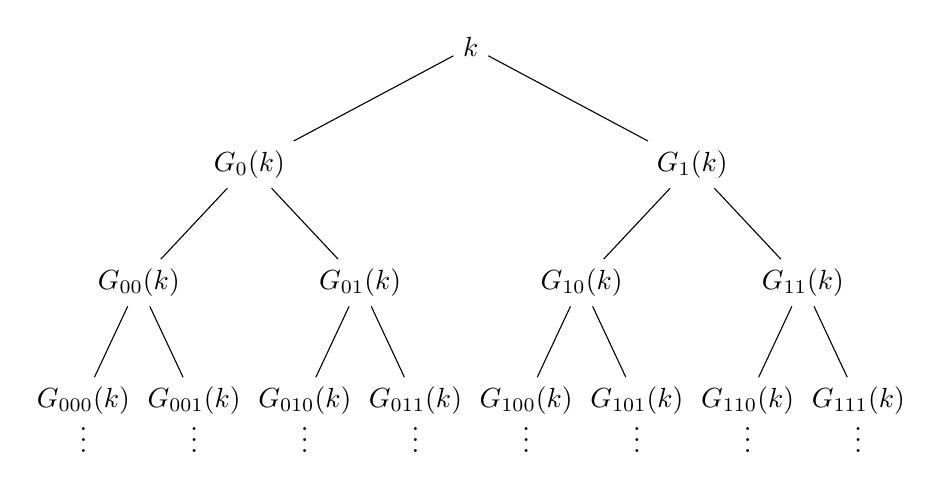
\begin{tikzpicture}[
            level 1/.style={sibling distance=16em},
            level 2/.style={sibling distance=8em},
            level 3/.style={sibling distance=4em}]

            \node{$k$}
                child{ node {$G_0(k)$}
                    child{ node {$G_{00}(k)$}
                        child{ node{$G_{000}(k)$} node[below]{$\vdots$}}
                        child{ node{$G_{001}(k)$} node[below]{$\vdots$}}
                    }
                    child{ node {$G_{01}(k)$}
                        child{ node{$G_{010}(k)$} node[below]{$\vdots$}}
                        child{ node{$G_{011}(k)$} node[below]{$\vdots$}}
                    }
                }
                child{ node {$G_1(k)$}
                    child{ node {$G_{10}(k)$}
                        child{ node{$G_{100}(k)$} node[below]{$\vdots$}}
                        child{ node{$G_{101}(k)$} node[below]{$\vdots$}}
                    }
                    child{ node {$G_{11}(k)$}
                        child{ node{$G_{110}(k)$} node[below]{$\vdots$}}
                        child{ node{$G_{111}(k)$} node[below]{$\vdots$}}
                    }
                };
        \end{tikzpicture}
        \caption{The \textsc{ggm}-tree for $G$}
        \label{fig:ggmtree}
    \end{figure}

\end{construction}

The proof of \prf-ness will be discussed in the next lesson.
